\documentclass[dvipsnames,usenames,aspectratio=169,12pt]{beamer}

% 日本語設定
\usepackage{zxjatype}
\usepackage[noto-jp]{zxjafont}

\usepackage{graphicx}
\usepackage{amsmath,amssymb}
\usepackage{url}

%\usetheme{metropolis}
%\usetheme{Execushares}
%\usetheme{modern}
%\usetheme{CodeCourse}
%\usetheme{focus}
%\usetheme{corporate}
\usetheme{cleancode}
%\usetheme[shape=circle]{LightTheme}

\usepackage{listings}
\lstset{
  basicstyle={\ttfamily},
  identifierstyle={\small},
  commentstyle={\smallitshape},
  keywordstyle={\small\bfseries},
  ndkeywordstyle={\small},
  stringstyle={\small\ttfamily},
  breaklines=true,
  columns=[l]{flexible},
}

\usepackage[yyyymmdd]{datetime}
\renewcommand{\dateseparator}{--}

\title{WSLとWindows Terminalの導入}
\author{濵田\,幸希}
\date{\today}

\begin{document}

\maketitle

\begin{frame}{今日やること}

基本的に資料を読んで進める(わからなければ呼んでください).

\vspace{10pt}

\begin{enumerate}
\item WSLをインストールする\\
\vspace{3pt}
設定が上手く出来ていなければ,アンインストールかリセット
\vspace{5pt}
\item Windows Terminalをインストールする
\vspace{5pt}
\item Windows Terminalの設定を行う
\end{enumerate}

\end{frame}

\begin{frame}{WSL(Windows Subsystem for Linux)とは}


要するに,\vspace{3pt}

Windows\,10上でLinuxを
「\alert{アプリケーション}」として動かすシステム.

\vspace{10pt}

\begin{quoteblock}{}[Wikipedia]
\begin{quote}
Windows Subsystem for Linux とは、Linuxのバイナリ実行ファイルをWindows 10およびWindows Server上でネイティブ実行するための互換レイヤーである。
\end{quote}
\end{quoteblock}

\end{frame}

\begin{frame}{対応しているLinuxディストリビューション}

現状,対応している種類が少ないので,実質\,\alert{Ubuntu}\,一択...

\vspace{10pt}
\begin{itemize}
\item Ubuntu
\vspace{5pt}
\item Debian GNU/Linux
\vspace{5pt}
\item Kali Linux
\vspace{5pt}
\item OpenSUSE Leap 42
\vspace{5pt}
\item Fedora Remix for WSL
\end{itemize}

\end{frame}

\begin{frame}{WSL2について}

\begin{itemize}
\item 従来(WSL1)
\vspace{5pt}

WSL1はLinuxを実際に動かしていたのではなく,Linuxの命令を\\\vspace{3pt}
Windowsの命令に\alert{変換}させていた.

\vspace{5pt}
\hspace{10pt}$\Longrightarrow$使用できないLinuxの機能やソフトウェアなどがあった.
\vspace{15pt}

\item WSL2では
\vspace{5pt}

\alert{Hyper-V}(Windows10の仮想化技術)を用いることで,実際にLinuxを\\\vspace{3pt}動かしている.

\vspace{5pt}
\hspace{10pt}$\Longrightarrow$今まで動かなかったソフトウェア(CCasl2等)やDockerなどが
\\\vspace{3pt}\hspace{32.5pt}使えるように!

\end{itemize}

\end{frame}

\begin{frame}{WSL2のデメリット}

\begin{itemize}
\item VirtualBoxのような他の仮想化ソフトウェアが\alert{使えなくなる}
\vspace{5pt}

WSL2はHyper-Vを使用するので,VirtualBoxなどと\alert{競合}してしまう.

\vspace{3pt}
(VMwareはWindows10をアップグレードしたら動く)

\vspace{15pt}

\item 使用し続けるとメモリが\alert{不足する}可能性がある
\vspace{5pt}

WSL2のプロセスVmmemがメモリを確保し続ける.

\vspace{5pt}
\hspace{10pt}$\Longrightarrow$ホスト側(Windows10)のメモリが足りなくなるかも・・・
\vspace{5pt}

メモリサイズを固定したり,手動で解放してあげたりなど
\\\vspace{3pt}といった暫定的な対策方法はある.

\end{itemize}

\end{frame}

\begin{frame}{Windows Terminalとは}

Microsoftが開発している\alert{ターミナルエミュレータ}.

\vspace{3pt}
コマンドプロンプトやPowerShell,WSLなどに対応している.

\begin{figure}[h]
\centering
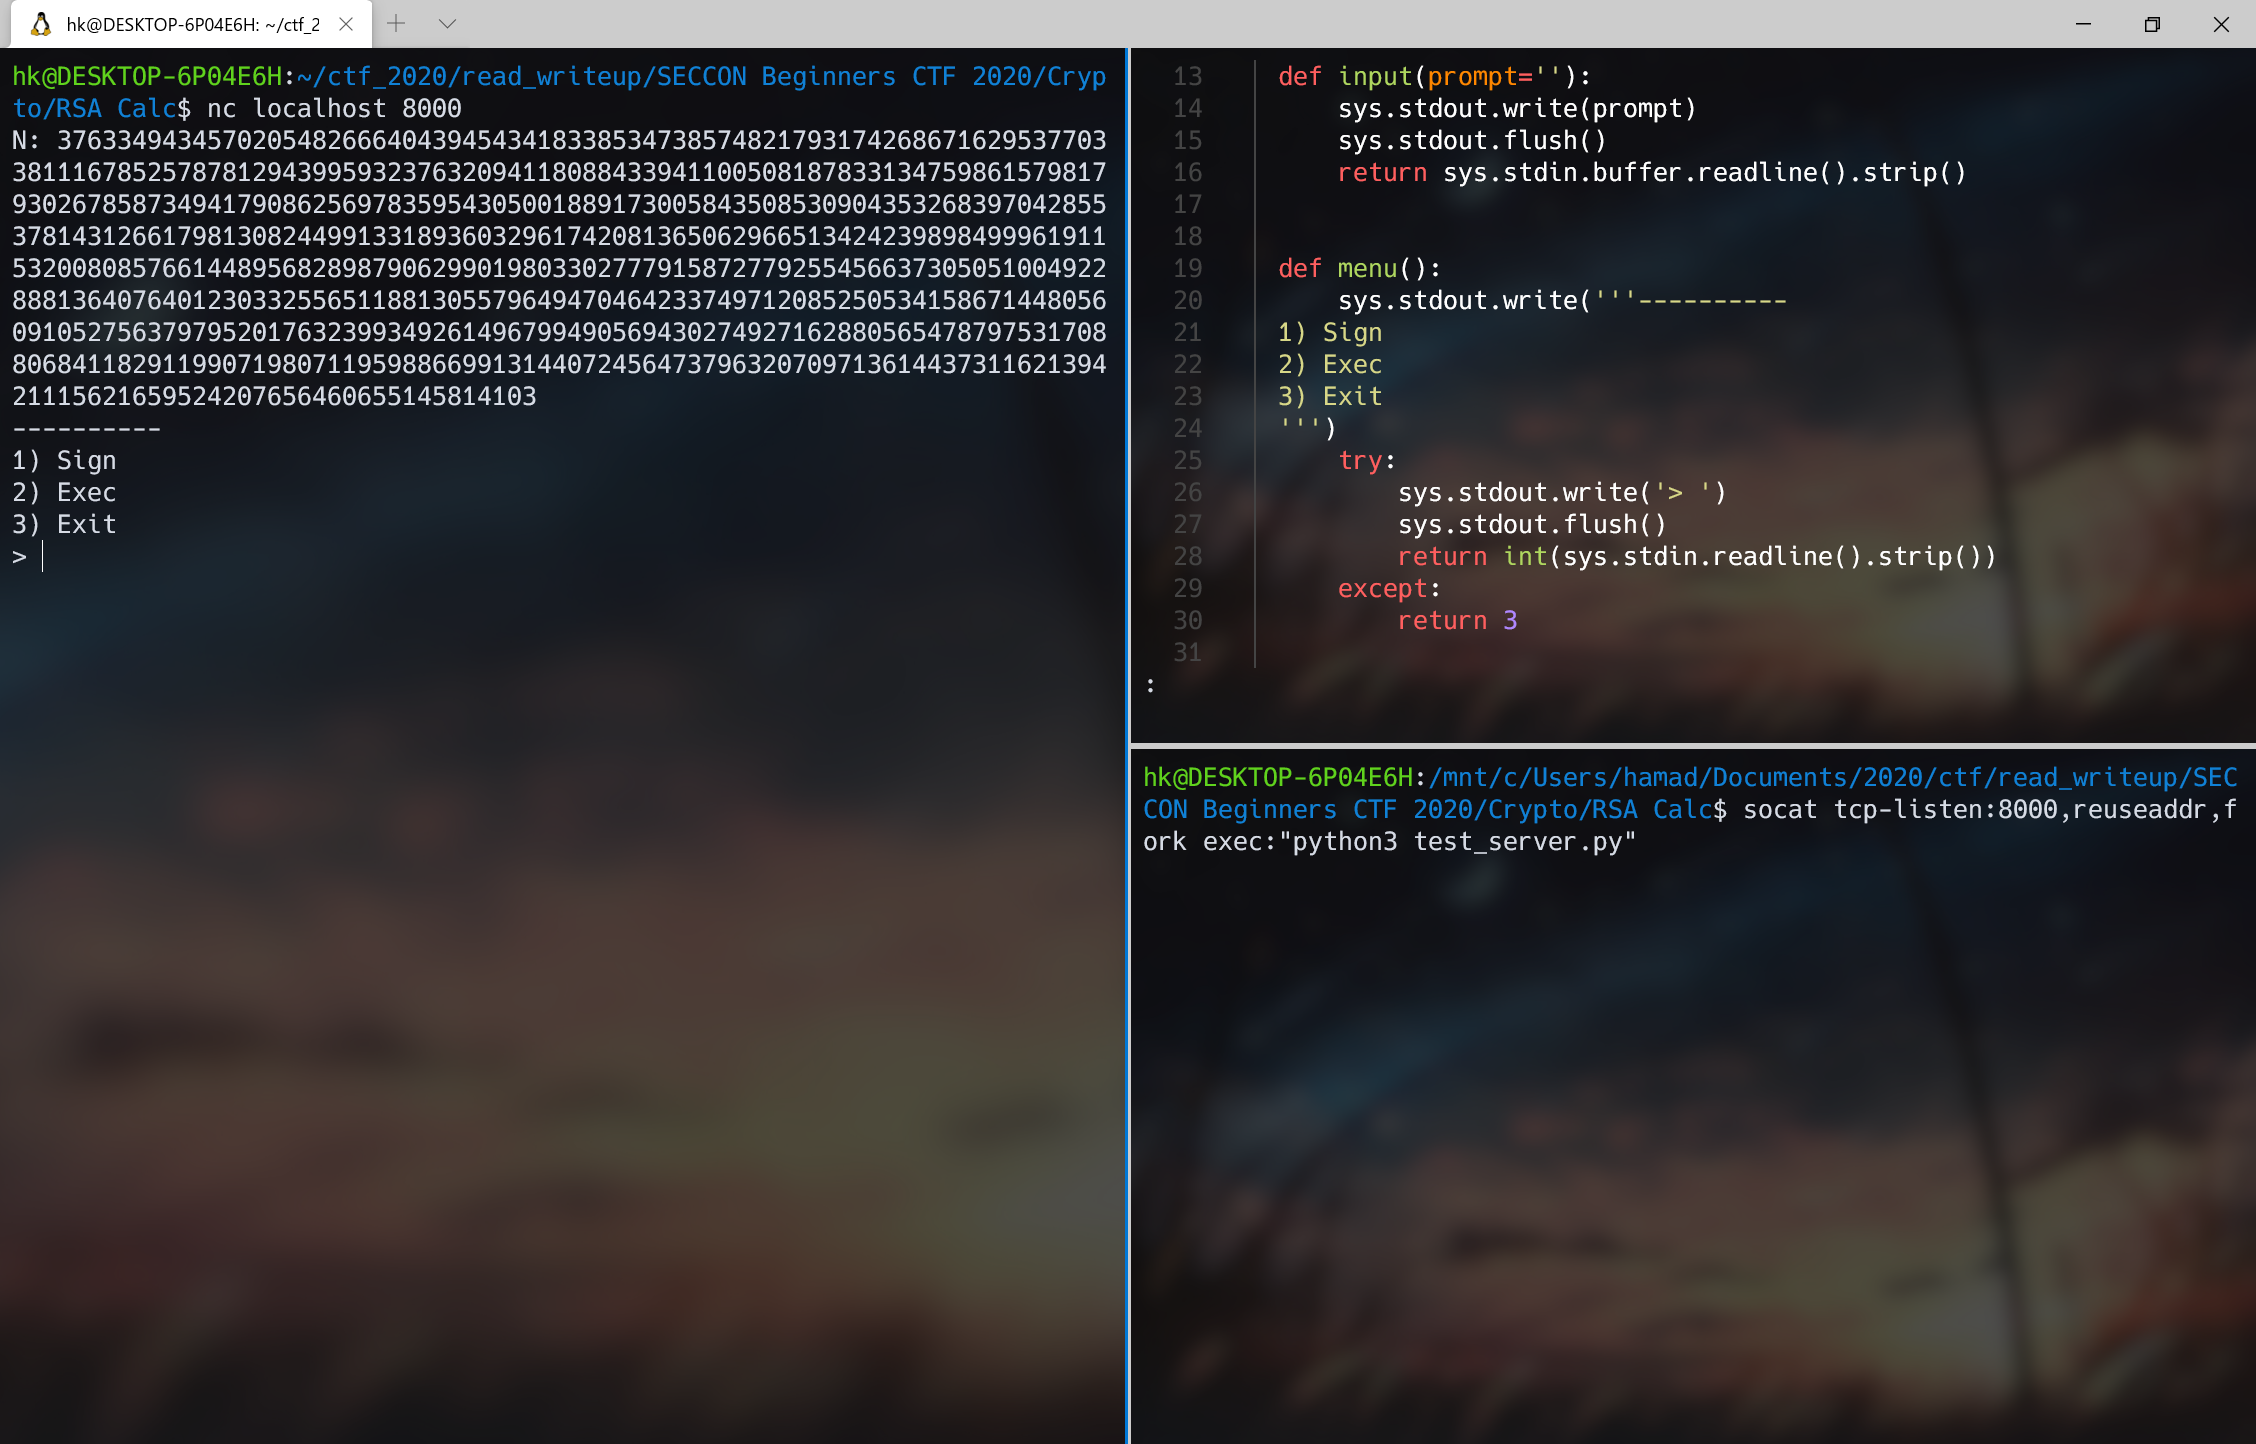
\includegraphics[scale=0.2]{./fig/myterminal.png}
\end{figure}
\end{frame}

\begin{frame}{公式ドキュメントがわかりやすい(一部,日本語対応)}
Microsoftが開発しているだけあって,公式ドキュメントが充実している!

\begin{figure}[h]
\centering
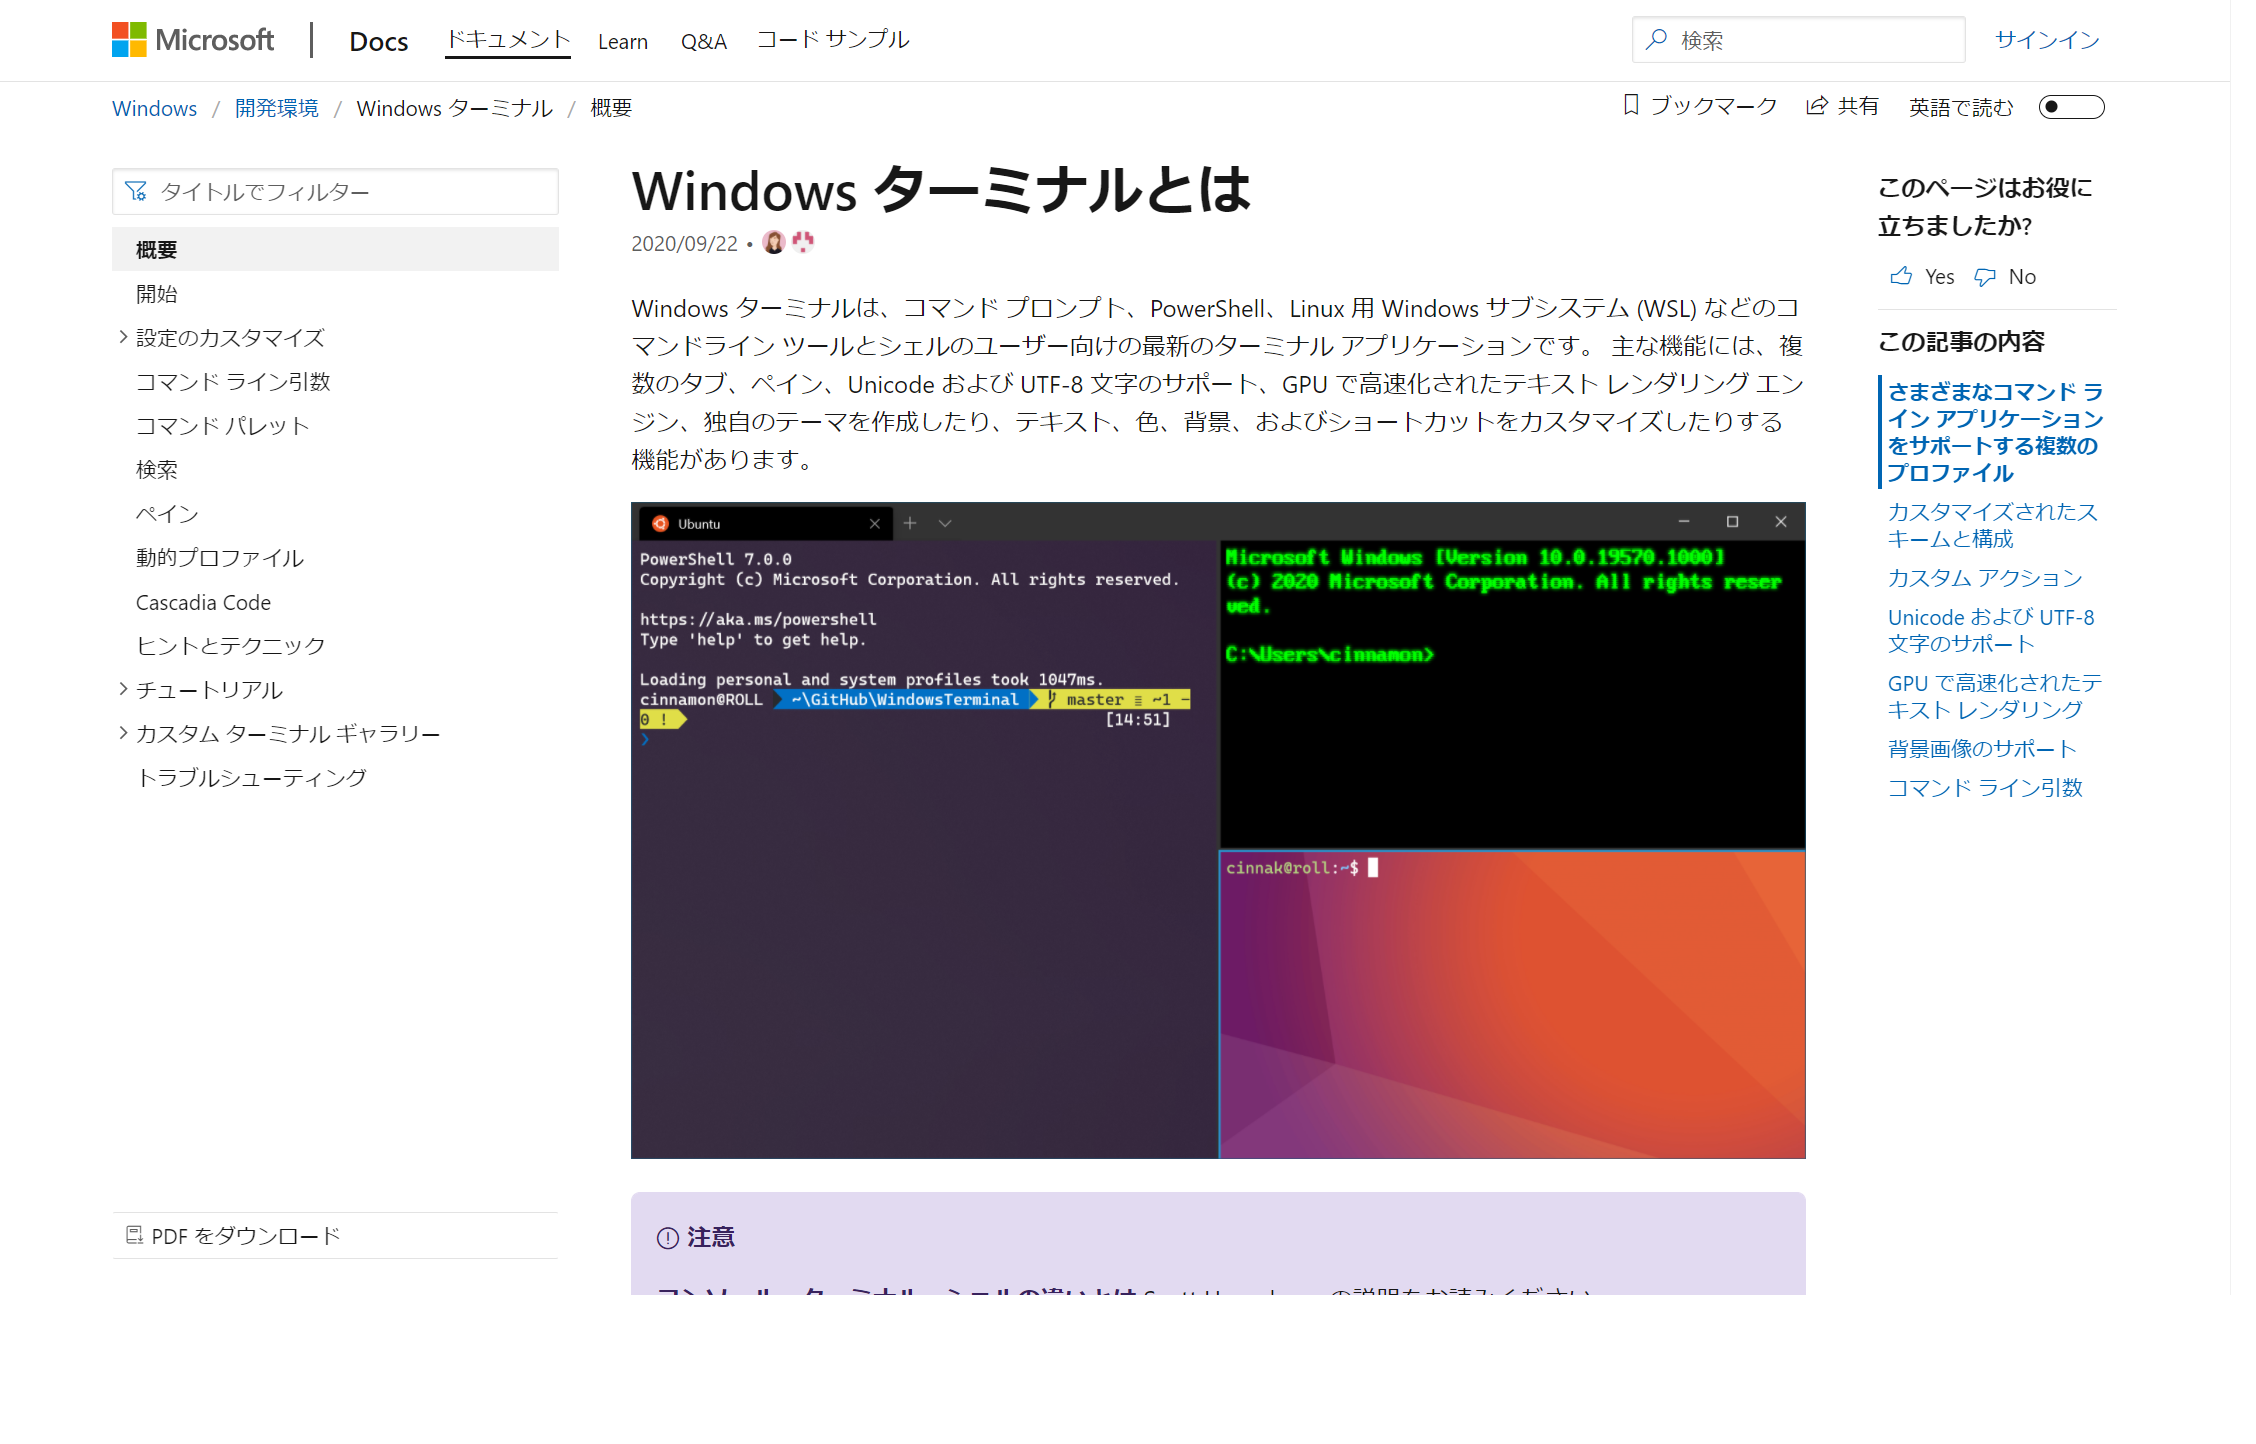
\includegraphics[scale=0.22]{./fig/docs.png}
\end{figure}
\end{frame}

\begin{frame}{色やショートカットキーなどの設定が簡単}
settings.jsonがとてもシンプルで楽!
\begin{figure}[h]
\centering
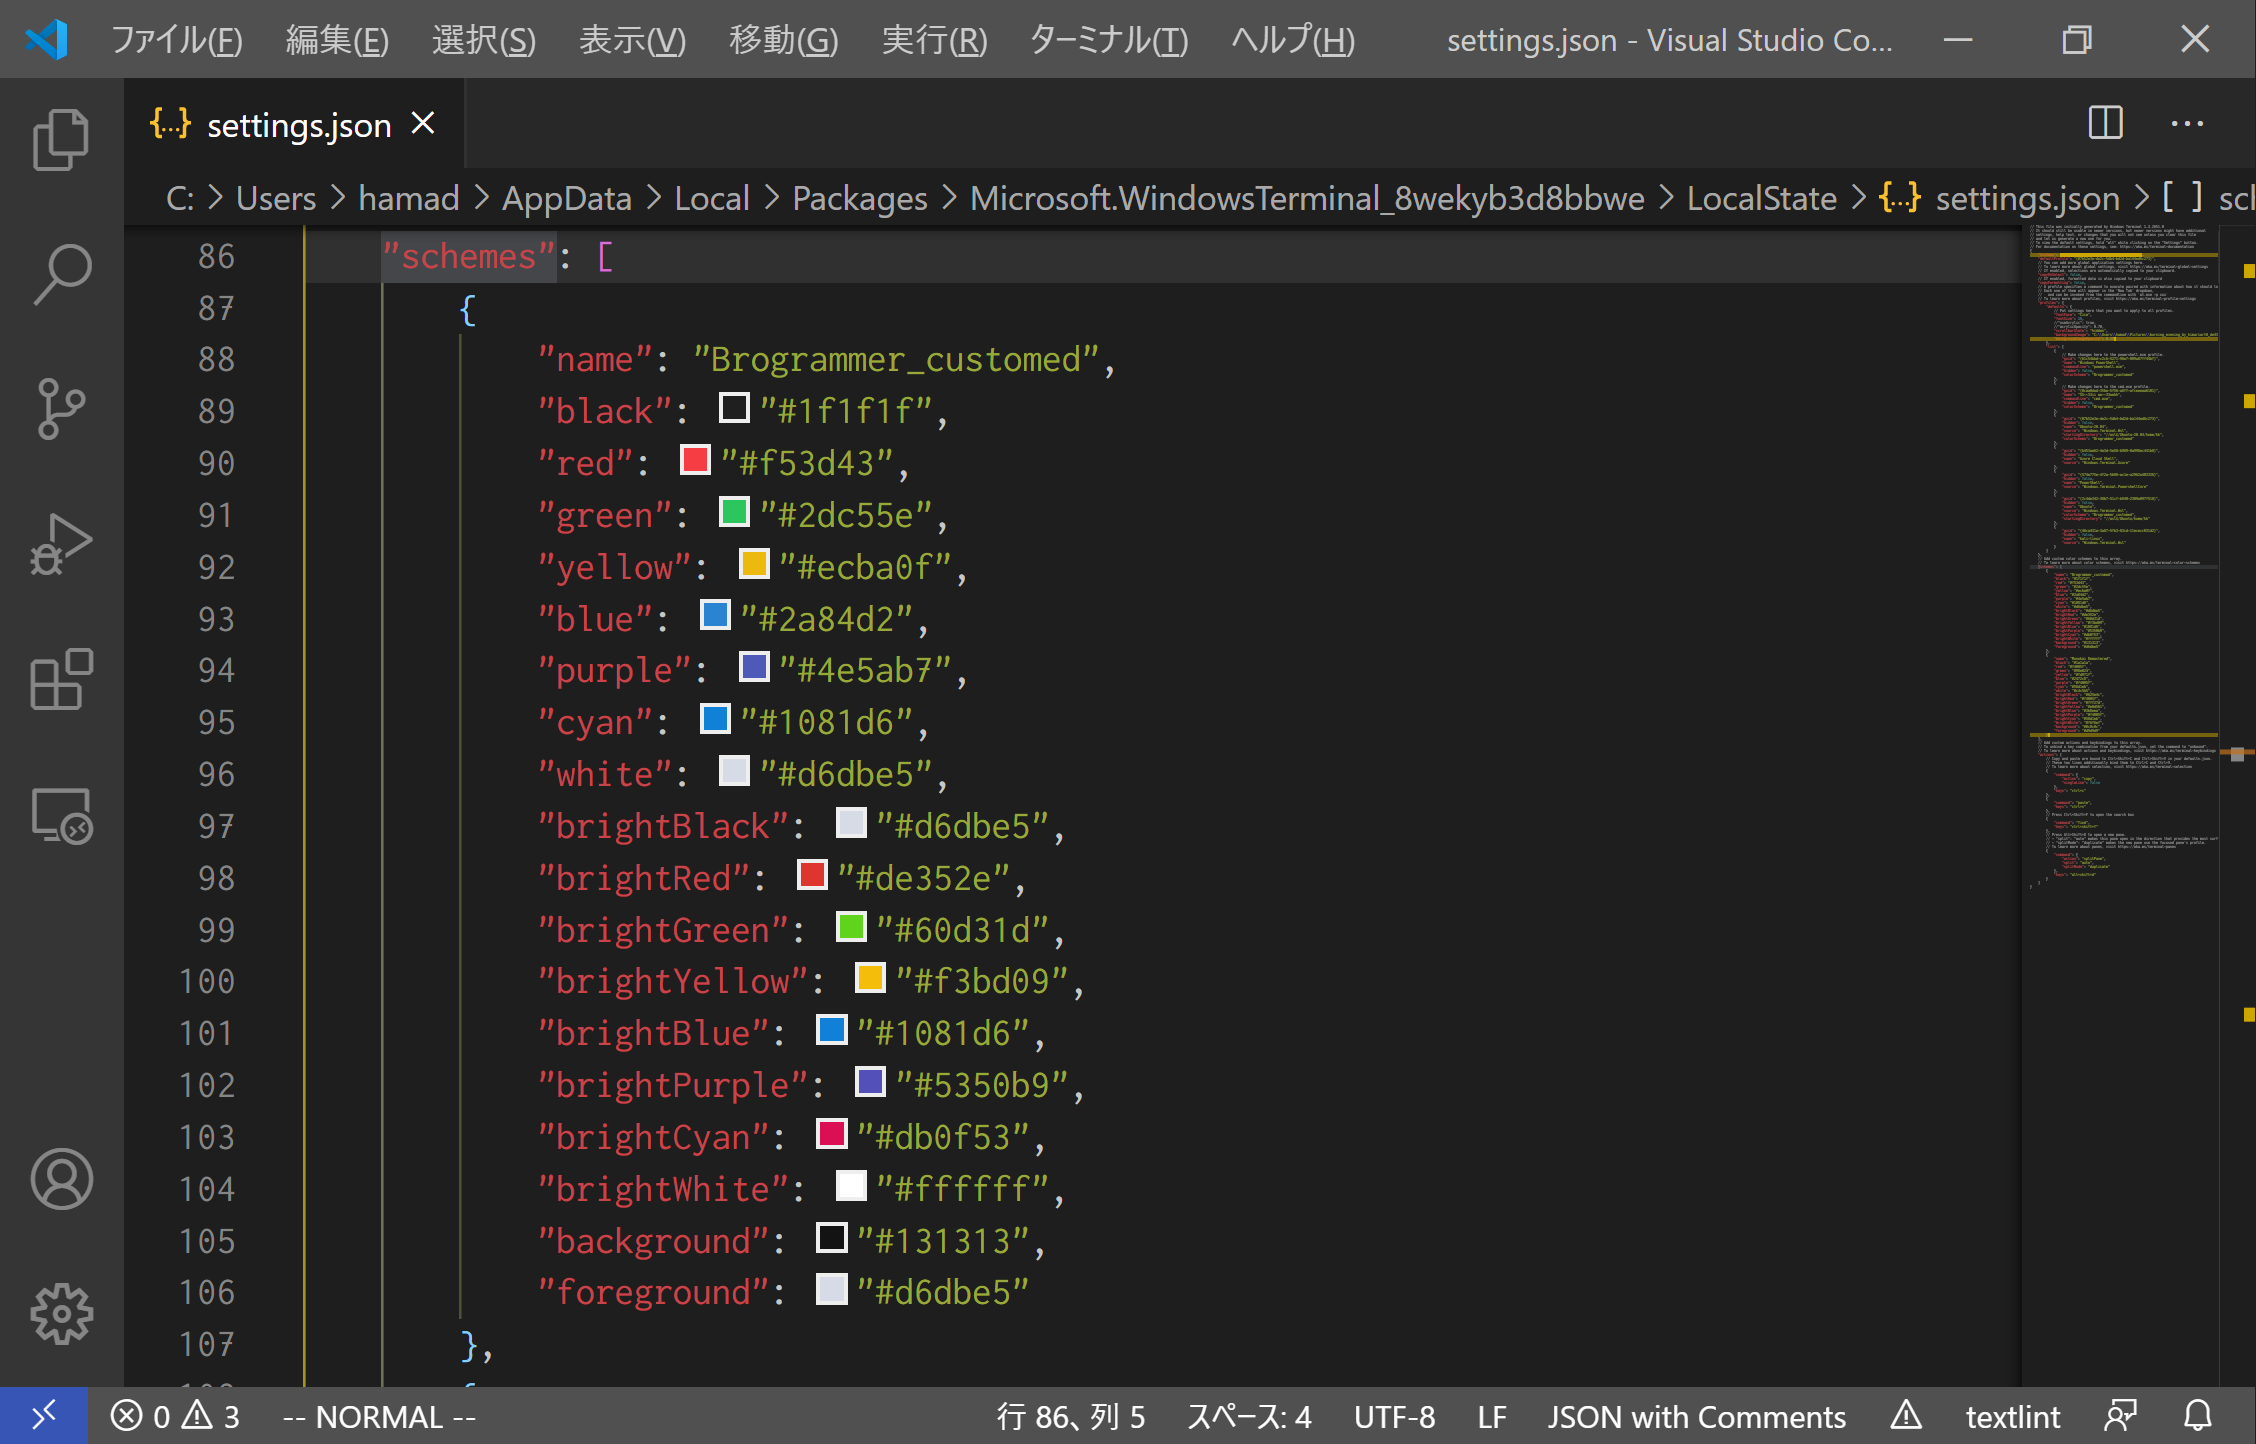
\includegraphics[scale=0.22]{./fig/color.png}
\end{figure}
\end{frame}
\end{document}